\documentclass[tikz,border=8pt]{standalone}
% Shared look for every TikZ diagram. Load with \input{../../tools/tikz-style.tex}
\usepackage[T1]{fontenc}
\usepackage{lmodern}
\renewcommand{\sfdefault}{lmr}  % diagrams use the same serif as the text
\usetikzlibrary{arrows.meta, positioning, shapes.geometric, calc, fit, backgrounds}
\definecolor{cblue}{HTML}{4C78A8}
\definecolor{corange}{HTML}{F58518}
\definecolor{cgreen}{HTML}{54A24B}
\definecolor{cred}{HTML}{E45756}
\definecolor{cpurple}{HTML}{B279A2}
\definecolor{cgrey}{HTML}{6B6B6B}
\tikzset{
  every picture/.style={font=\sffamily, line width=1.2pt},
  box/.style={draw=#1, fill=#1!12, rounded corners=4pt, align=center, inner sep=7pt, minimum height=1.1cm},
  box/.default=cgrey,
  arrow/.style={-{Stealth[length=3mm]}, draw=cgrey, line width=1.4pt},
  title/.style={font=\sffamily\bfseries\Large},
  note/.style={font=\sffamily\small, text=cgrey, align=center},
}
\AtBeginDocument{\hyphenpenalty=10000 \exhyphenpenalty=10000}

% Shapes of the full and the thin (reduced) SVD of a tall m x n matrix (m = 3, n = 2 drawn as 6 x 4 blocks).
\newcommand{\blk}[6]{ % x, y, w, h, colour, label
  \draw[draw=#5, fill=#5!15, line width=1.2pt] (#1,#2) rectangle ++(#3,#4);
  \node[font=\Large] at ($(#1,#2)+0.5*(#3,#4)$) {#6};
}
\begin{document}
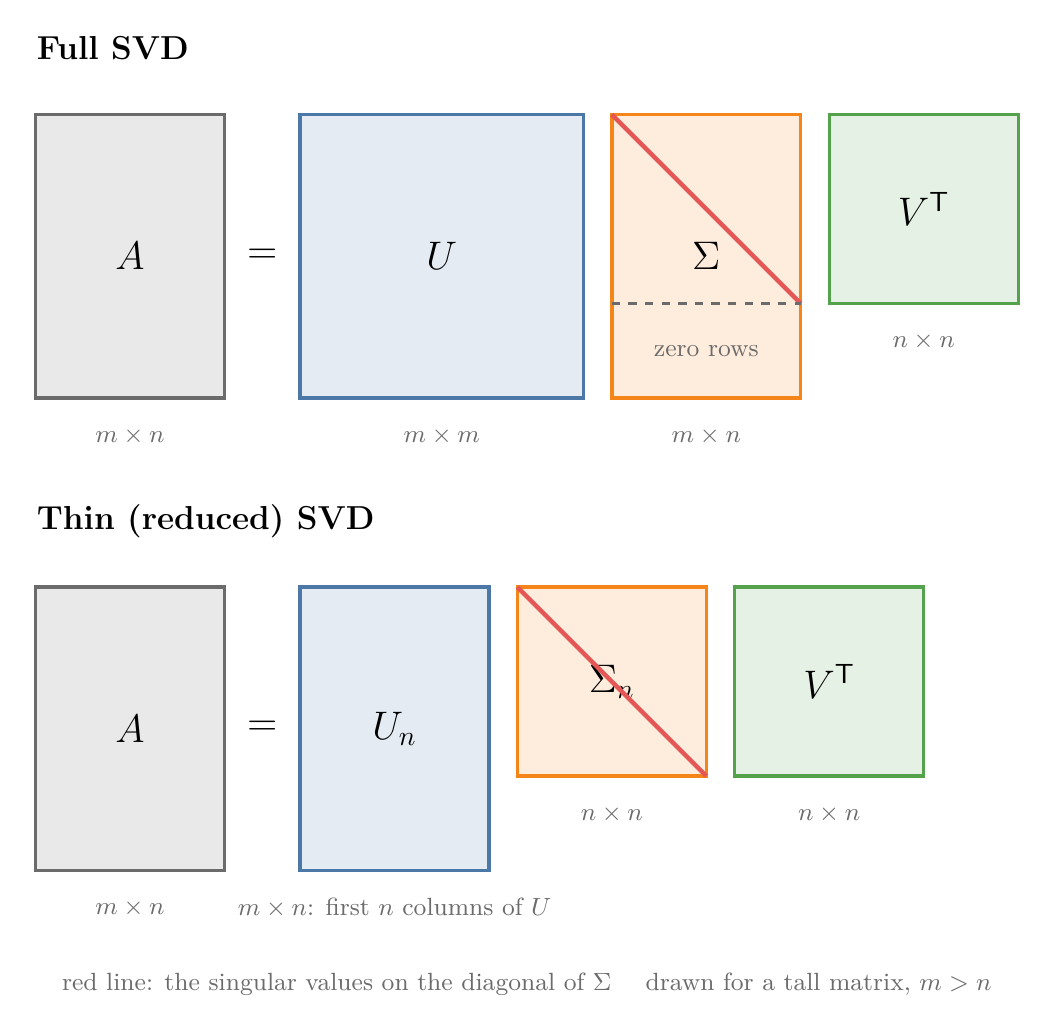
\begin{tikzpicture}[scale=0.6]
  % full
  \node[font=\bfseries\large, anchor=west] at (-0.2,7.4) {Full SVD};
  \blk{0}{0}{4}{6}{cgrey}{$A$}
  \node[font=\Large] at (4.8,3) {$=$};
  \blk{5.6}{0}{6}{6}{cblue}{$U$}
  \blk{12.2}{0}{4}{6}{corange}{$\Sigma$}
  \draw[cred, line width=1.6pt] (12.2,6) -- (16.2,2);
  \draw[cgrey, dashed, line width=0.8pt] (12.2,2) -- (16.2,2);
  \node[note] at (14.2,1) {zero rows};
  \blk{16.8}{2}{4}{4}{cgreen}{$V^{\mathsf T}$}
  \node[note] at (2,-0.8) {$m \times n$};
  \node[note] at (8.6,-0.8) {$m \times m$};
  \node[note] at (14.2,-0.8) {$m \times n$};
  \node[note] at (18.8,1.2) {$n \times n$};
  % thin
  \begin{scope}[yshift=-10cm]
    \node[font=\bfseries\large, anchor=west] at (-0.2,7.4) {Thin (reduced) SVD};
    \blk{0}{0}{4}{6}{cgrey}{$A$}
    \node[font=\Large] at (4.8,3) {$=$};
    \blk{5.6}{0}{4}{6}{cblue}{$U_n$}
    \blk{10.2}{2}{4}{4}{corange}{$\Sigma_n$}
    \draw[cred, line width=1.6pt] (10.2,6) -- (14.2,2);
    \blk{14.8}{2}{4}{4}{cgreen}{$V^{\mathsf T}$}
    \node[note] at (2,-0.8) {$m \times n$};
    \node[note] at (7.6,-0.8) {$m \times n$: first $n$ columns of $U$};
    \node[note] at (12.2,1.2) {$n \times n$};
    \node[note] at (16.8,1.2) {$n \times n$};
  \end{scope}
  \node[note] at (10.4,-12.4) {red line: the singular values on the diagonal of $\Sigma$ \quad drawn for a tall matrix, $m > n$};
\end{tikzpicture}
\end{document}
